\documentclass[10pt,twocolumn,letterpaper]{article}

\usepackage{cvpr}
\usepackage{times}
\usepackage{epsfig}
\usepackage{graphicx}
\usepackage{amsmath}
\usepackage{amssymb}



% Include other packages here, before hyperref.

% If you comment hyperref and then uncomment it, you should delete
% egpaper.aux before re-running latex.  (Or just hit 'q' on the first latex
% run, let it finish, and you should be clear).
\usepackage[breaklinks=true,bookmarks=false]{hyperref}

\cvprfinalcopy % *** Uncomment this line for the final submission

\def\cvprPaperID{****} % *** Enter the CVPR Paper ID here
\def\httilde{\mbox{\tt\raisebox{-.5ex}{\symbol{126}}}}

% Pages are numbered in submission mode, and unnumbered in camera-ready
%\ifcvprfinal\pagestyle{empty}\fi
\setcounter{page}{1}
\begin{document}

%%%%%%%%% TITLE
\title{3D Object Detection and Tracking using Graph Neural Networks on Waymo Dataset}

\author{Ahmed Bahnasy\\
Technical University in Munich\\

{\tt\small ahmed.bahnasy@tum.de}
% For a paper whose authors are all at the same institution,
% omit the following lines up until the closing ``}''.
% Additional authors and addresses can be added with ``\and'',
% just like the second author.
% To save space, use either the email address or home page, not both
}

\maketitle
%\thispagestyle{empty}

%%%%%%%%% ABSTRACT
\begin{abstract}
Recent approaches for 3D object detection have made a tremendous progress due to the development of deep learning. this also highly influences the  progress in other tasks like 3D Multi-object tracking (MOT) which is an indispensable component to any autonomous system. Recent work uses a standard tracking- by-detection pipeline, where feature extraction is first per- formed independently for each object in order to compute an affinity matrix. Then the affinity matrix is passed to the Hungarian algorithm for data association. This matching can be seen as discrete optimisation process and there is no learning it. A key factor of this standard pipeline is to learn discriminative features for different objects, by relying on a robust detector in order to reduce confusion during data association. In this task, we experiment with improving the discriminative feature learning for MOT: by first build a robust object detector and second instead of obtaining features for each object independently, we try applying learning module for tracking by introducing the Graph Neural Network which enables feature interaction mechanism. As a result, the feature of one object is informed of the features of other objects so that the object feature can lean towards the object with similar feature (i.e., object probably with a same ID) and deviate from objects with dissimilar features (i.e., object prob- ably with different IDs), leading to a more discriminative feature for each object
\end{abstract}

%%%%%%%%% BODY TEXT
\section{Introduction}

\paragraph{}
Robust 3D perception becomes an essential component in any state-of-the-art autonomous system. 3D detection has a series of challenges: First, point-clouds are sparse, the points are unevenly distributed across the 3D space, and most of the 3D space are without measurements. Second, 3D objects have a wide range of sizes, shapes and aspect ratios, for example, in autonomous driving domain, buses, trucks and cars are elongated, pedestrians are tall and cyclists are nearly planer. These challenges makes applying ideas from 2D domain to 3D domain not straight forward. trying to use the anchor based approach followed in 2D domain by assigning a different anchor for each object orientation increases the computational cost and may introduce a large number of of potential false-positive detections. the main challenge for linking up 2D and 3D domains lies in the way the objects are represented \cite{yang20203dssd}. representing objects as points greatly simplifies 3D recognition \cite{yin2020center}. In this task, we tried to build a 3D that detects centers of the objects and their properties using a key-point detector \cite{zhou2019objects}. In specific we followed the same approach in \cite{yin2020center, ge2020afdet} by using any standard Lidar-based backbone network, for example, PointPillars or VoxelNet, to build an intermediate representation for the input point cloud. this representation is then flattened into Birds-Eye-View map using a standard image-based key-point detector to find object centers \cite{zhou2019objects}. the rest of the 3D bounding box parameters, i.e., 3D Size, orientation, and velocity, are then regressed from the center location vector. according to \cite{yin2020center}, center-based representation has several advantages: First, it reduces the detector search space since points has no orientation, unlike bounding boxes. Second, center-based representation simplifies the tracking downstream tasks. 

\paragraph{}
Much like 3D perception, Multi-object tracking (MOT) is a crucial component for autonomous driving \cite{luo2018fast}. Tracking-by-detection paradigm is the dominant approach when it comes to online MOT problems \cite{bewley2016simple, weng2019baseline}. The main idea is to apply object detector to all frames and extract features independently from each detected object. Then pairwise similarity is computed between objects and a Hungarian algorithm \cite{kuhn1955hungarian} is used to solve the problem. The key idea in this approach is to learn discriminative features for the objects with different identities to reduce the confusion in the matching. One key observation is that feature extraction is done independently and there is no interaction between features during feature extraction. according to \cite{weng2020gnn3dmot}, independent feature extraction is sub-optimal for discriminative feature learning. this idea is very important for MOT, given the fact that an object in current frame can be matched to at most one object in the previous frame. so if the similarity between two features increased, then the pairwise similarity between the rest of the objects and any of these two objects should be decreased to avoid confusion for matching. based on that observation, we followed \cite{weng2020gnn3dmot} by implementing a Graph Neural Network to do the feature interaction. The idea is to construct a graph with each node being the object feature. Then, each node can update its feature by aggregating features from other nodes during layer propagation step. the object feature is now not isolated and can be adapted with respect to other features.
%-------------------------------------------------------------------------

\section{Related Work}

\paragraph{3D Object Detection} is all about predicting the three dimensional rotated bounding boxes \cite{geiger2012we, lang2019pointpillars, qi2018frustum, yan2018second, yang20203dssd, yang2019std}. Most 3D-based methods either use point cloud data directly or require converting these data into 3D grids or voxels instead of generating BEV representations. In \cite{wang2015voting}, point cloud data are converted into voxels containing feature vectors, and then a novel convolution-like voting-based algorithm is used for detection. Vote3Deep \cite{engelcke2017vote3deep} leverages feature voting in \cite{wang2015voting} to efficiently process the sparse 3D point-cloud in equally spaced 3D voxels. VoxelNet \cite{zhou2018voxelnet} uses a PointNet \cite{qi2017pointnet} inside each voxel to generate a unified feature representation from which a head with 3D sparse convolutions \cite{graham20183d} and 2D convolutions produces detections. SECOND \cite{yan2018second} simplifies the VoxelNet and speeds up sparse 3D convolutions. PIXOR \cite{yang2018pixor} project all points onto a 2D feature map with 3D occupancy and point intensity information to remove the expensive 3D convolutions. PointPillars\cite{lang2019pointpillars} replaces all voxel computation with a pillar representation, a single tall elongated voxel per map location, improving backbone efficiency. MVF \cite{zhou2020end} and Pillar-od \cite{wang2020pillar} combine multiple view features to learn a more effective pillar representation. In this task we followed \cite{yin2020center, ge2020afdet} by focusing on the output representation and employ any 3D encoder to get the representation.

\paragraph{Online Multi-Object Tracking} is mostly addressed using Tracking by Detection paradigm. the performance is highly impacted by two factors: object detection quality and discriminative feature learning. After the affinity matrix is computed based on the pairwise similarity of learned discriminative feature, the problem of online MOT could be addressed as as a discrete optimization problem and could be solved using as  bipartite matching problem using the Hungarian algorithm \cite{kuhn1955hungarian}. To obtain discriminative feature, prior work mostly focuses on the feature selection. Among different features, it turns out that motion and appearance are the most dis- criminative features. Early work employs hand-crafted features such as spatial distance \cite{pirsiavash2011globally} and Intersection of Union (IoU) \cite{bochinski2017high} as the motion feature, and use color histograms as the appearance feature. Recently, Convolutional Neural Networks have been used to extract appearance feature \cite{baser2019fantrack, frossard2018end}. Regarding the motion feature, many filter based approaches has been used \cite{bewley2016simple, weng2019baseline}. Deep learning approaches has been introduced for motion feature in \cite{baser2019fantrack}. we followed the same idea in \cite{wojke2017simple, weng2020gnn3dmot} by exploring both the appearance and motion feature with focus on the 3D space.

\paragraph{Graph Neural Networks} is used as way to improve discriminative feature learning for MOT after showing promising performance in many fields\cite{hamilton2017inductive,velivckovic2017graph,kipf2016semi, berg2017graph, monti2017geometric, ying2018graph}. GNNs was first proposed by \cite{gori2005new} to directly process graph-structured data using neural networks. The major component of the GNNs is the node feature aggregation technique, with which node can update its feature by interacting with other nodes. With this technique, significant success has been achieved in many fields using GNNs such as semantic segmentation\cite{chen2019graph}, action recognition \cite{shi2019skeleton}, single object tracking \cite{gao2019graph}, person re-identification \cite{wu2019unsupervised}, point cloud classification and segmentation \cite{wang2019dynamic}. The majority of the work deals with object features as independent and isolated from other features. by leveraging node aggregation technique of the GNNs, object features could be iteratively evolved so that the feature of different objects can be more discriminative. the idea of feature interaction was first introduced in \cite{hu2018relation} to encode context information for object detection in the spatial domain, Although a temporal relation network is proposed in the follow-up work \cite{xu2019spatial}, the feature of a tracked object is only aggregating from its past trajectory and no interaction with other object features exist. in This task we followed \cite{yin2020center} by implementing a generic feature interaction framework that can model any kind of interaction in both spatial and temporal domains


%-------------------------------------------------------------------------

\section{Dataset}

%-------------------------------------------------------------------------

\section{Network Architecture}

During the early stages of this task, we tried to use Votenet \cite{qi2019deep} as 3D object detector. Despite the promising results of this architecture on Indoor dataset, it performs very poorly on outdoor datasets like KITTI and Waymo. More information about these experiments are stated Appendix \ref{appendix:votenet}

\subsection{Detection}

\subsection{Tracking}

%-------------------------------------------------------------------------

\section{Experiments}
\subsection{Main Results}
\subsection{Ablation Studies}

\if false
All manuscripts must be in English.

\subsection{Dual submission}

Please refer to the author guidelines on the CVPR 2020 web page for a
discussion of the policy on dual submissions.

\subsection{Paper length}
Papers, excluding the references section,
must be no longer than eight pages in length. The references section
will not be included in the page count, and there is no limit on the
length of the references section. For example, a paper of eight pages
with two pages of references would have a total length of 10 pages.
{\bf There will be no extra page charges for CVPR 2020.}

Overlength papers will simply not be reviewed.  This includes papers
where the margins and formatting are deemed to have been significantly
altered from those laid down by this style guide.  Note that this
\LaTeX\ guide already sets figure captions and references in a smaller font.
The reason such papers will not be reviewed is that there is no provision for
supervised revisions of manuscripts.  The reviewing process cannot determine
the suitability of the paper for presentation in eight pages if it is
reviewed in eleven.  

%-------------------------------------------------------------------------
\subsection{The ruler}
The \LaTeX\ style defines a printed ruler which should be present in the
version submitted for review.  The ruler is provided in order that
reviewers may comment on particular lines in the paper without
circumlocution.  If you are preparing a document using a non-\LaTeX\
document preparation system, please arrange for an equivalent ruler to
appear on the final output pages.  The presence or absence of the ruler
should not change the appearance of any other content on the page.  The
camera ready copy should not contain a ruler. (\LaTeX\ users may uncomment
the \verb'\cvprfinalcopy' command in the document preamble.)  Reviewers:
note that the ruler measurements do not align well with lines in the paper
--- this turns out to be very difficult to do well when the paper contains
many figures and equations, and, when done, looks ugly.  Just use fractional
references (e.g.\ this line is $095.5$), although in most cases one would
expect that the approximate location will be adequate.

\subsection{Mathematics}

Please number all of your sections and displayed equations.  It is
important for readers to be able to refer to any particular equation.  Just
because you didn't refer to it in the text doesn't mean some future reader
might not need to refer to it.  It is cumbersome to have to use
circumlocutions like ``the equation second from the top of page 3 column
1''.  (Note that the ruler will not be present in the final copy, so is not
an alternative to equation numbers).  All authors will benefit from reading
Mermin's description of how to write mathematics:
\url{http://www.pamitc.org/documents/mermin.pdf}.


\subsection{Blind review}

Many authors misunderstand the concept of anonymizing for blind
review.  Blind review does not mean that one must remove
citations to one's own work---in fact it is often impossible to
review a paper unless the previous citations are known and
available.

Blind review means that you do not use the words ``my'' or ``our''
when citing previous work.  That is all.  (But see below for
techreports.)

Saying ``this builds on the work of Lucy Smith [1]'' does not say
that you are Lucy Smith; it says that you are building on her
work.  If you are Smith and Jones, do not say ``as we show in
[7]'', say ``as Smith and Jones show in [7]'' and at the end of the
paper, include reference 7 as you would any other cited work.

An example of a bad paper just asking to be rejected:
\begin{quote}
\begin{center}
    An analysis of the frobnicatable foo filter.
\end{center}

   In this paper we present a performance analysis of our
   previous paper [1], and show it to be inferior to all
   previously known methods.  Why the previous paper was
   accepted without this analysis is beyond me.

   [1] Removed for blind review
\end{quote}


An example of an acceptable paper:

\begin{quote}
\begin{center}
     An analysis of the frobnicatable foo filter.
\end{center}

   In this paper we present a performance analysis of the
   paper of Smith \etal [1], and show it to be inferior to
   all previously known methods.  Why the previous paper
   was accepted without this analysis is beyond me.

   [1] Smith, L and Jones, C. ``The frobnicatable foo
   filter, a fundamental contribution to human knowledge''.
   Nature 381(12), 1-213.
\end{quote}

If you are making a submission to another conference at the same time,
which covers similar or overlapping material, you may need to refer to that
submission in order to explain the differences, just as you would if you
had previously published related work.  In such cases, include the
anonymized parallel submission~\cite{Authors14} as additional material and
cite it as
\begin{quote}
[1] Authors. ``The frobnicatable foo filter'', F\&G 2014 Submission ID 324,
Supplied as additional material {\tt fg324.pdf}.
\end{quote}

Finally, you may feel you need to tell the reader that more details can be
found elsewhere, and refer them to a technical report.  For conference
submissions, the paper must stand on its own, and not {\em require} the
reviewer to go to a techreport for further details.  Thus, you may say in
the body of the paper ``further details may be found
in~\cite{Authors14b}''.  Then submit the techreport as additional material.
Again, you may not assume the reviewers will read this material.

Sometimes your paper is about a problem which you tested using a tool which
is widely known to be restricted to a single institution.  For example,
let's say it's 1969, you have solved a key problem on the Apollo lander,
and you believe that the CVPR70 audience would like to hear about your
solution.  The work is a development of your celebrated 1968 paper entitled
``Zero-g frobnication: How being the only people in the world with access to
the Apollo lander source code makes us a wow at parties'', by Zeus \etal.

You can handle this paper like any other.  Don't write ``We show how to
improve our previous work [Anonymous, 1968].  This time we tested the
algorithm on a lunar lander [name of lander removed for blind review]''.
That would be silly, and would immediately identify the authors. Instead
write the following:
\begin{quotation}
\noindent
   We describe a system for zero-g frobnication.  This
   system is new because it handles the following cases:
   A, B.  Previous systems [Zeus et al. 1968] didn't
   handle case B properly.  Ours handles it by including
   a foo term in the bar integral.

   ...

   The proposed system was integrated with the Apollo
   lunar lander, and went all the way to the moon, don't
   you know.  It displayed the following behaviours
   which show how well we solved cases A and B: ...
\end{quotation}
As you can see, the above text follows standard scientific convention,
reads better than the first version, and does not explicitly name you as
the authors.  A reviewer might think it likely that the new paper was
written by Zeus \etal, but cannot make any decision based on that guess.
He or she would have to be sure that no other authors could have been
contracted to solve problem B.
\medskip

\noindent
FAQ\medskip\\
{\bf Q:} Are acknowledgements OK?\\
{\bf A:} No.  Leave them for the final copy.\medskip\\
{\bf Q:} How do I cite my results reported in open challenges?
{\bf A:} To conform with the double blind review policy, you can report results of other challenge participants together with your results in your paper. For your results, however, you should not identify yourself and should not mention your participation in the challenge. Instead present your results referring to the method proposed in your paper and draw conclusions based on the experimental comparison to other results.\medskip\\



\begin{figure}[t]
\begin{center}
\fbox{\rule{0pt}{2in} \rule{0.9\linewidth}{0pt}}
   %\includegraphics[width=0.8\linewidth]{egfigure.eps}
\end{center}
   \caption{Example of caption.  It is set in Roman so that mathematics
   (always set in Roman: $B \sin A = A \sin B$) may be included without an
   ugly clash.}
\label{fig:long}
\label{fig:onecol}
\end{figure}

\subsection{Miscellaneous}

\noindent
Compare the following:\\
\begin{tabular}{ll}
 \verb'$conf_a$' &  $conf_a$ \\
 \verb'$\mathit{conf}_a$' & $\mathit{conf}_a$
\end{tabular}\\
See The \TeX book, p165.

The space after \eg, meaning ``for example'', should not be a
sentence-ending space. So \eg is correct, {\em e.g.} is not.  The provided
\verb'\eg' macro takes care of this.

When citing a multi-author paper, you may save space by using ``et alia'',
shortened to ``\etal'' (not ``{\em et.\ al.}'' as ``{\em et}'' is a complete word.)
However, use it only when there are three or more authors.  Thus, the
following is correct: ``
   Frobnication has been trendy lately.
   It was introduced by Alpher~\cite{Alpher02}, and subsequently developed by
   Alpher and Fotheringham-Smythe~\cite{Alpher03}, and Alpher \etal~\cite{Alpher04}.''

This is incorrect: ``... subsequently developed by Alpher \etal~\cite{Alpher03} ...''
because reference~\cite{Alpher03} has just two authors.  If you use the
\verb'\etal' macro provided, then you need not worry about double periods
when used at the end of a sentence as in Alpher \etal.

For this citation style, keep multiple citations in numerical (not
chronological) order, so prefer \cite{Alpher03,Alpher02,Authors14} to
\cite{Alpher02,Alpher03,Authors14}.


\begin{figure*}
\begin{center}
\fbox{\rule{0pt}{2in} \rule{.9\linewidth}{0pt}}
\end{center}
   \caption{Example of a short caption, which should be centered.}
\label{fig:short}
\end{figure*}

%------------------------------------------------------------------------
\section{Formatting your paper}

All text must be in a two-column format. The total allowable width of the
text area is $6\frac78$ inches (17.5 cm) wide by $8\frac78$ inches (22.54
cm) high. Columns are to be $3\frac14$ inches (8.25 cm) wide, with a
$\frac{5}{16}$ inch (0.8 cm) space between them. The main title (on the
first page) should begin 1.0 inch (2.54 cm) from the top edge of the
page. The second and following pages should begin 1.0 inch (2.54 cm) from
the top edge. On all pages, the bottom margin should be 1-1/8 inches (2.86
cm) from the bottom edge of the page for $8.5 \times 11$-inch paper; for A4
paper, approximately 1-5/8 inches (4.13 cm) from the bottom edge of the
page.

%-------------------------------------------------------------------------
\subsection{Margins and page numbering}

All printed material, including text, illustrations, and charts, must be kept
within a print area 6-7/8 inches (17.5 cm) wide by 8-7/8 inches (22.54 cm)
high.
Page numbers should be in footer with page numbers, centered and .75
inches from the bottom of the page and make it start at the correct page
number rather than the 4321 in the example.  To do this fine the line (around
line 23)
\begin{verbatim}
%\ifcvprfinal\pagestyle{empty}\fi
\setcounter{page}{4321}
\end{verbatim}
where the number 4321 is your assigned starting page.

Make sure the first page is numbered by commenting out the first page being
empty on line 46
\begin{verbatim}
%\thispagestyle{empty}
\end{verbatim}


%-------------------------------------------------------------------------
\subsection{Type-style and fonts}

Wherever Times is specified, Times Roman may also be used. If neither is
available on your word processor, please use the font closest in
appearance to Times to which you have access.

MAIN TITLE. Center the title 1-3/8 inches (3.49 cm) from the top edge of
the first page. The title should be in Times 14-point, boldface type.
Capitalize the first letter of nouns, pronouns, verbs, adjectives, and
adverbs; do not capitalize articles, coordinate conjunctions, or
prepositions (unless the title begins with such a word). Leave two blank
lines after the title.

AUTHOR NAME(s) and AFFILIATION(s) are to be centered beneath the title
and printed in Times 12-point, non-boldface type. This information is to
be followed by two blank lines.

The ABSTRACT and MAIN TEXT are to be in a two-column format.

MAIN TEXT. Type main text in 10-point Times, single-spaced. Do NOT use
double-spacing. All paragraphs should be indented 1 pica (approx. 1/6
inch or 0.422 cm). Make sure your text is fully justified---that is,
flush left and flush right. Please do not place any additional blank
lines between paragraphs.

Figure and table captions should be 9-point Roman type as in
Figures~\ref{fig:onecol} and~\ref{fig:short}.  Short captions should be centred.

\noindent Callouts should be 9-point Helvetica, non-boldface type.
Initially capitalize only the first word of section titles and first-,
second-, and third-order headings.

FIRST-ORDER HEADINGS. (For example, {\large \bf 1. Introduction})
should be Times 12-point boldface, initially capitalized, flush left,
with one blank line before, and one blank line after.

SECOND-ORDER HEADINGS. (For example, { \bf 1.1. Database elements})
should be Times 11-point boldface, initially capitalized, flush left,
with one blank line before, and one after. If you require a third-order
heading (we discourage it), use 10-point Times, boldface, initially
capitalized, flush left, preceded by one blank line, followed by a period
and your text on the same line.

%-------------------------------------------------------------------------
\subsection{Footnotes}

Please use footnotes\footnote {This is what a footnote looks like.  It
often distracts the reader from the main flow of the argument.} sparingly.
Indeed, try to avoid footnotes altogether and include necessary peripheral
observations in
the text (within parentheses, if you prefer, as in this sentence).  If you
wish to use a footnote, place it at the bottom of the column on the page on
which it is referenced. Use Times 8-point type, single-spaced.


%-------------------------------------------------------------------------
\subsection{References}

List and number all bibliographical references in 9-point Times,
single-spaced, at the end of your paper. When referenced in the text,
enclose the citation number in square brackets, for
example~\cite{Authors14}.  Where appropriate, include the name(s) of
editors of referenced books.

\begin{table}
\begin{center}
\begin{tabular}{|l|c|}
\hline
Method & Frobnability \\
\hline\hline
Theirs & Frumpy \\
Yours & Frobbly \\
Ours & Makes one's heart Frob\\
\hline
\end{tabular}
\end{center}
\caption{Results.   Ours is better.}
\end{table}

%-------------------------------------------------------------------------
\subsection{Illustrations, graphs, and photographs}

All graphics should be centered.  Please ensure that any point you wish to
make is resolvable in a printed copy of the paper.  Resize fonts in figures
to match the font in the body text, and choose line widths which render
effectively in print.  Many readers (and reviewers), even of an electronic
copy, will choose to print your paper in order to read it.  You cannot
insist that they do otherwise, and therefore must not assume that they can
zoom in to see tiny details on a graphic.

When placing figures in \LaTeX, it's almost always best to use
\verb+\includegraphics+, and to specify the  figure width as a multiple of
the line width as in the example below
{\small\begin{verbatim}
   \usepackage[dvips]{graphicx} ...
   \includegraphics[width=0.8\linewidth]
                   {myfile.eps}
\end{verbatim}
}


%-------------------------------------------------------------------------
\subsection{Color}

Please refer to the author guidelines on the CVPR 2020 web page for a discussion
of the use of color in your document.

%------------------------------------------------------------------------
\section{Final copy}

You must include your signed IEEE copyright release form when you submit
your finished paper. We MUST have this form before your paper can be
published in the proceedings.

Please direct any questions to the production editor in charge of these 
proceedings at the IEEE Computer Society Press: 
\url{https://www.computer.org/about/contact}. 
\fi

{\small
\bibliographystyle{ieee_fullname}
\bibliography{egbib}
}


\appendix
\section*{Appendices}
\addcontentsline{toc}{section}{Appendices}
\renewcommand{\thesubsection}{\Alph{subsection}}

\subsection{Votenet for Lidar Outdoor Scenes}\label{apendix:votenet}

\subsubsection {Data preparation and Training}
VoteNet consists of two modules: the proposal module which consumes the raw point cloud and produces the virtual voting points; and the object proposal and classification module that operates on the voting points to propose and classify objects. Up to now, VoteNet has only been tuned and tested on RGB-D data (ScanNet and SUN RGB-D). in order to adapt the model for Waymo, we implemented a custom input pipeline to optimally preprocess and feed the Waymo point cloud data into the VoteNet network.
Following the same train/validation/test split from Waymo paper \cite{cite waymo}, and following the same training procedure mentioned in \cite{votenet}, For each scene we randomly subsample 20k points. The scenes are furthermore augmented on-the-fly with random flips in horizontal plane, random uniform rotations along up-axis in  $\pm$30$^{\circ}$ range, and random uniform scaling of $\pm$10\%. In addition to three Euclidean coordinates for each point, we also include up to two additional features: the provided laser reflection intensities, and a height estimate for each point. The latter is estimated as a 1\% percentile of all point positions along the up-axis.
We perform training on the dynamic classes of the Waymo dataset: car, pedestrian, and cyclist. We choose one size template per class, and 12 bins for the heading angle. We train with a batch size of 16 and incorporate a scheduled learning policy with a starting LR of 0.001 and LR-decays by 0.1 at 60, 90, and 120 epochs, as well as an exponential BN momentum decay. We use same loss function as in SUN RGB-D case.
\paragraph{}
Points clouds from outdoor LiDAR scans are quite different from point clouds from RGB-D indoor scans. For example, the typical scales of the Waymo scenes are significantly larger than those of indoor scans, with depth fields reaching beyond 70 meters along forward-axis. the LiDAR point cloud has strongly varying density and is generally more sparse than the point clouds produced from the RGB-D imagery. Point features extracted from sparse regions may generalize poorly to dense regions, and vice versa

to further adapt VoteNet to the distinct characteristics of the outdoor LiDAR scenes. we adapt the receptive field radii and increase the number of clusters for feature aggregation. to capture fine details of point cloud and, at the same time, mitigate  the corruption of local patterns due to sampling deficiency in sparse cloud regions, we enhance the set-abstraction modules of the backbone network with multi-scale grouping (MSG) layers \cite{pointnet++}, which concatenate features at different scales before feeding them into the feature aggregation layer.

Among all the experiments to find the best backbone network parameters, we ended up following the configuration in \cite{RCNN paper} by configuring four MSG-based SA layers used to subsample the inputs to 4096, 1024, 256 and 64 points, and two FP layers to upsample the points back to 1024 points, each with additional 512 deep features. Tables \ref{tab:votenet_oringinal} and \ref{tab:votenet_msg} illustrates the difference between the two backbones.


\begin{table*}
\label{tab:votenet_oringinal}
\begin{center}
\begin{tabular}{|c|c|c|c|c|}
\hline
Module (Input) & Output dimensions & clusters K & Receptive field radius & MLP layer dimensions \\
\hline\hline
SA1 (PC) & (4096, 3 + 96) & 2048 & 0.2 & 64/64/128 \\
SA2 (SA1) & (1024, 3 + 256) & 1024 & 0.4 & 128/128/256 \\
SA3 (SA2) & (512, 3 + 512) & 512 & 0.8 & 128/128/256 \\
SA4 (SA3) & (64, 3 + 512) & 256 & 1.2 & 128/128/256 \\
FC1 (SA3, SA4) & (512, 3 + 512) & - & - & 512/512 \\
FC2 (SA2, SA3) & (1024, 3 + 512) & - & - & 512/512 \\
\hline
\end{tabular}
\end{center}
\caption{Original Architecture of VPN in \cite{votenet paper}}
\end{table*}



\begin{table*}
\label{tab:votenet_msg}
\begin{center}
\begin{tabular}{|c|c|c|c|c|}
\hline
Module (Input) & Output dimensions & clusters K & MSG Radii & MLP layers \\
\hline\hline
SA1 (PC) & (4096, 3 + 96) & 2048 & 0.1,  0.5 & 16/16/32, 32/32/64 \\
SA2 (SA1) & (1024, 3 + 256) & 1024 & 0.1,  0.5 & 64/64/128,  64/96/128 \\
SA3 (SA2) & (512, 3 + 512) & 512 & 0.1,  0.5 & 128/196/256,  128/196/256 \\
SA4 (SA3) & (64, 3 + 512) & 256 & 0.1,  0.5 & 256/256/512,  256/256/512 \\
FC1 (SA3, SA4) & (512, 3 + 512) & - & - & 512/512 \\
FC2 (SA2, SA3) & (1024, 3 + 512) & - & - & 512/512 \\
\hline
\end{tabular}
\end{center}
\caption{Enhanced architecture of VPN with two MSG radii of receptive fields $r_{1,2}$ (meters), and MLP parameters for each MSG group implemented \cite{RCNN paper}}
\end{table*}

\subsubsection{Results on 360$^{\circ}$ Point cloud}
When working the 360 point cloud, the Average Precision results from different VoteNet architectures were very poor. after training for nearly 120 epochs, mAP over the test set was nearly 0.15 only. the problem lies in the different points densities between outdoor LiDAR point clouds and  indoor RGB-D point cloud. there are a lot of objects which have only 2 ~ 10 points per bounding box. after the initial downsampling from 120k to 20k points for processing the further downsampling done by Set abstraction modules, the final proposal points are actually lie outside most of the ground truth bounding boxes as shown in Figure \ref{fig:proposal_points}. Thus, the network was not able to learn the correct voting. nearly all of the detected objects in this experiment were objects near to the sensor with >= 1000 points, all objects with fewer points were missed.

\begin{figure}
	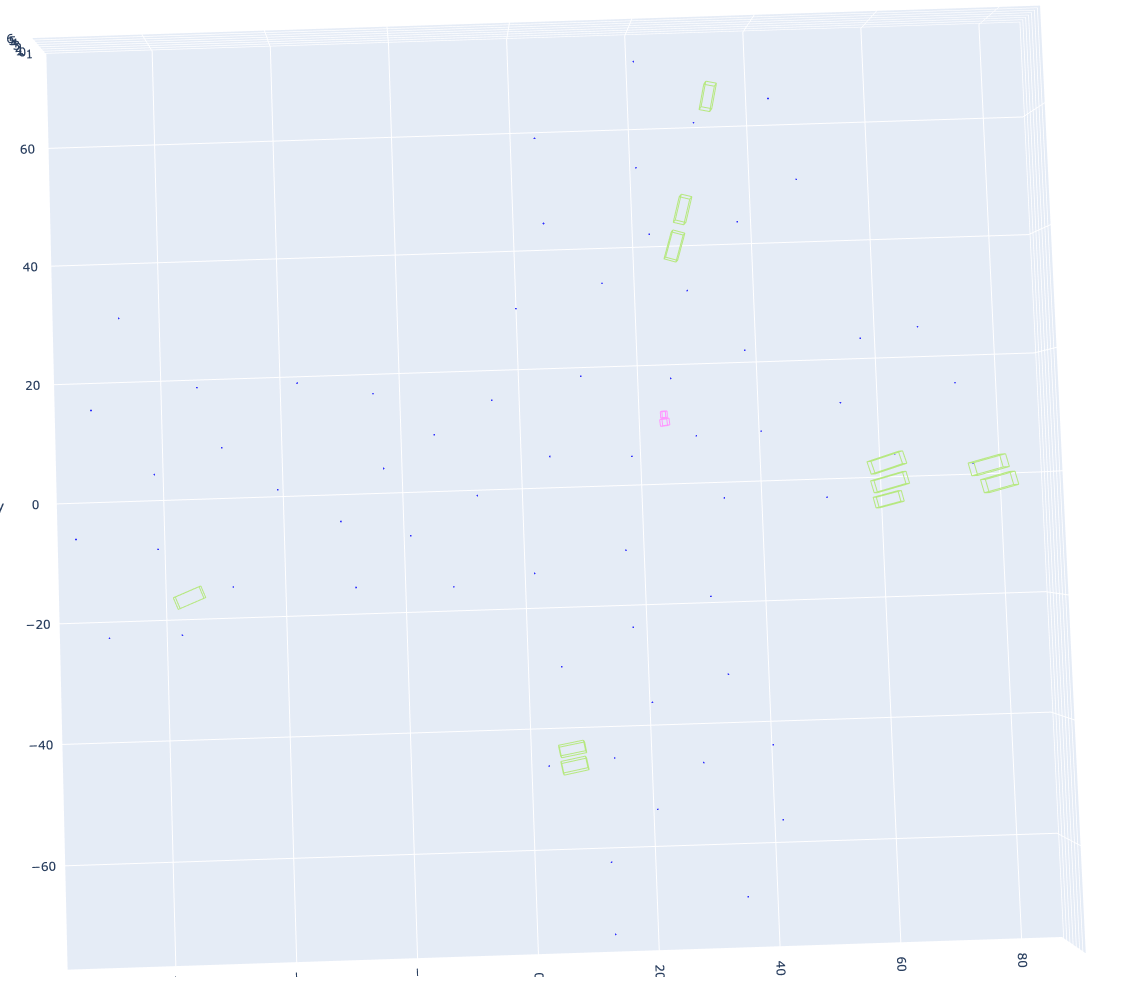
\includegraphics[width=\linewidth]{media/votenet_proposal_points.png}
   \caption{Top view of final 3D space. Blue Points are the final proposal points from VoteNet. Green and Magenta boxes are Ground truth bounding boxes. During training, the final proposal are all lie outside the ground truth bounding boxes. Hence, the voting module cannot learn the correct modules.}
\label{fig:proposal_points}
\end{figure}

\subsubsection{Results on Front Camera Frustum Point Cloud}
To verify the results of the previous section, we did an extensive exploration in the literature about the experiments involves raw point processing approaches \cite{pointnet, point++, votennet, votenet frustutm, point rcnn} for outdoor datasets \cite{KITTI,  nuscenes, Waymo, a2d2}. interesting work in \cite{point rcnn} in forground background segmentation caught our attention. as a first step, we reproduced the work in \cite{point RCNN} on KITTI dataset \cite{KITTI}. Then, Before reproducing the same experiment on Waymo \ cite{}, we implemented a specific data processing pipeline to make Waymo point cloud identical to KITTI. As KITTI includes annotations only for the objects in teh front camera frustum. we first project the 360-degree LiDAR data onto the image plane and extract the point cloud that lie inside the result- ing frustum. This step reduces the average number on points per scene from $\sim$170k to 16,384. For each scene we randomly subsample 16,384 points, and for scenes with fewer points, we randomly copy the points up to a total of 16,384.

reducing the size of the point cloud make a tremendous boost in the (AP) results of VoteNet when we re-executed the experimetents mentioned in \ref{} on this data setup. due to the small initial input size, the ratio between points inside bounding boxes to the points outside bounding boxes are very large when compared in case of using the 360 point cloud. many of the final proposal points are found inside the ground truth bounding boxes. Thus the voting module was able to learn the correct voting. Figure \ref{fig:votnet_front_camera_results} shows the final results of running two VoteNet architectures on the reduced Waymo point clouds.

\begin{figure}
	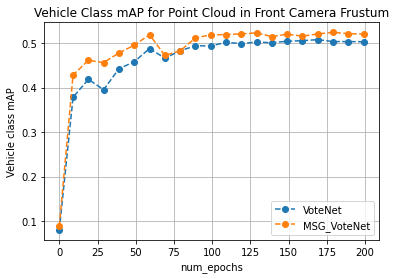
\includegraphics[width=\linewidth]{media/votenet_mAP.png}
   \caption{Example of caption.  It is set in Roman so that mathematics
   (always set in Roman: $B \sin A = A \sin B$) may be included without an
   ugly clash.}
\label{fig:votnet_front_camera_results}
\end{figure}


\subsection{Appendix Two Test}

Minkowski Vs Spconv vs Sparse Tensor library


\end{document}
